\section{Structured Based Measurement}
\label{sec:SBM}
% The problems of first view, what second view could fix it
By Interpretation Based Measurement in section \ref{sec:IBM}, similarity between predicates is obtained, and used to answer queries in a fuzzy way.  For example, as known, \textit{Beautiful} and \textit{Popular} have a high similarity value, querying \textit{popular(X)}, not only returns results from \textit{popular(X)}, but also from \textit{Beautiful(X)} . In this way, fuzzy query-answering gives more similar choices for users. However, concepts in real world, such as ``geek''  and ``unsociable'' share a large amount of people in each group, by Interpretation Based Measurement, they would be connected with higher similarity value, but semantically, they don't refer to similar concepts according to their linguistics definitions.  In this case, asking for ``geek'', the ``computer scientist''  returns, so does ``unsociable", asking for ``unsociable'', ``shy people'' returns, so does ``geek". Obviously, not only those real similar concepts are gained, but some untruthful results are obtained at the same time, since Interpretation Based Measurement builds strong similarity between ``unsociable'' and ``geek''. In order to avoid this disadvantage, we propose Structured Based Measurement, in which similarity between predicates is defined from their embedded meanings. In RFuzzy Framework, the embedded meaning of predicate is presented by its structure.

In Structured Based Measurement, we build a tree for each predicate, so comparing two predicates is indeed comparing two trees. Section \ref{sec:PredicateTree} introduces the approach to build a tree for predicate. In section \ref{sec:Algorithm}, the algorithm to obtain similarity between two trees is described in detail and its complexity is presented in section \ref{sec:Complexity}. 
\subsection{Predicate tree}
\label{sec:PredicateTree}
Firstly, the question of ``how to build a tree for a predicate in \textit{RFuzzy} Program" is the main focus. For convenience, the corresponding tree for the predicate is called as a \textit{predicate tree}. The first step is transforming an \textit{RFuzzy} Program, to obtain the subset of program which is used to create the predicate tree in section \ref{sec:TransformRFuzzy}. The approach of constructing predicate trees from subset of program is presented in section \ref{sec:Construct}. In {SBM} method, to be able to compare two predicate trees, the structure of the concerning trees should be the same. Moreover they ought to preserve the embedded meanings. To ensure this, the concept ``equivalent trees" is introduced in section \ref{sec:EquivalentTree}. According to ``equivalent trees", the predicate tree could be constructed with \textit{identities}, which is claimed to maintain the semantic meaning but reform the structure. This is described in section \ref{sec:ReConstruct}.

\subsubsection{Transforming RFuzzy program}
\label{sec:TransformRFuzzy}
In an \textit{RFuzzy program} $P=(R,D,T)$, $R$ is a set of \textit{fuzzy clauses}, $D$ is a set of \textit{default value declarations} and $T$ is a set of \textit{type declarations}. In order to construct a tree for each predicate in $P$, there is the need of filtering and reforming some parts of $P$. This procedure is called \textit{transformation}, in which two steps are taken, one is filtering and the other is reforming. In this section, the details \textit{how} and \textit{why} are presented \cite{Lu}. 

The result of first step \textit{filtering} is a tuple $P'=(R',D',T')$, which is generated from $P$ by following constrains,
\begin{enumerate}
 \item Refined $R'$

    $R$ as a set of \textit{fuzzy clauses}, includes fuzzy clauses, which are written as, \[A \stackrel{c,F_c}{\longleftarrow}F(B_1,...,B_n)\]
    where $A \in TB_{\Pi,\Sigma,V}$ is called the head, $B_1,...,B_n \in TB_{\Pi,\Sigma,V}$ is called the body, $c\in[0,1]$ is the credibility value, and $F_c\in\{\&_1,...,\&_k\}\subset\Omega^{(2)}$ and $F\in\Omega^{(n)}$ are connectives symbols. $F_c$ is to combine the credibility of the rule and the truth value of the body. $F$ is to combine the truth values of the subgoals in the body.
   
    A \textit{fuzzy fact} is a special case where $c=1$, $F_c$ is the usual product of real numbers  `` . ''  , $n=0$, $F\in\Omega^{(0)}$. It is written as \[A \longleftarrow v\]
    where $c$ and $F_c$ are omitted. 

    The similarity between predicates is a relevant value of comparison between two predicates, rather than the absolute value described in \textit{fuzzy facts}. Therefore, \textit{fuzzy facts} is out of consideration of similarity between predicates.
    
    As a result, $R'$ is a set of all \textit{fuzzy clauses}, but not \textit{fuzzy facts}, notated as, $R'=R\backslash R_{facts}$.
 \item Refined $D'$

    A \textit{default value declaration} for a predicate $p \in \Pi ^{(n)}$ is written as 
    \begin{center}
       $default(p/n)=[\delta_1$ if $\varphi_1$, ..., $\delta_m$ if $\varphi_m]$
    \end{center}
    where $\delta_i\in[0,1]$ for all $i$. The $\varphi_i$ are first-order formulas restricted to terms in $p$ from $TU_{\Sigma,V_p}$, the predicates $=$ and $\neq$, the symbol true and the junctors $\wedge$ and $\vee$ in their usual meaning, which are \textit{`and'}, \textit{ `or'}.

    There is a special case called \textit{unconditional} default value declaration where $m=1$ and $\varphi_1=true$ in the default value declarations. In this case, the predicate $p/n$ is not related to any other predicates,  and therefore it is out of consideration in similarity.

    All in all, $D'$ is all the \textit{conditional} default value declarations, notated as, $D'=D\backslash D_{unconditional}$.

 \item Refined $T'$
    
    \[T=T_{term} \cup T_{predicate}\]
    $T_{term}$ is a set of all \textit{term type declarations}, which assign a type $\tau \in \mathcal{T}$ to a term $t \in \mathbb{HU}$ and is written as $t : \tau$. $T_{predicate}$ is a set of all predicate type declarations. A \textit{predicate type declaration} assigns a type $(\tau_1,...,\tau_n) \in \mathcal{T}^n$ to predicate $p\in\Pi^n$ and is written as $p : (\tau_1,...,\tau_n)$, where $\tau_i$ is the type of $p$'s $i$-th argument.

    The $T_{term}$ is not related to predicates at all, so it is not taken into account of the similarity between predicates.

    Therefore, $T'=T_{predicate}$.
 \end{enumerate}

After filtering the RFuzzy program $P=(R,D,T)$ into $P'=(R',D',T')$, the second step is taken to reform $D'$ into $D_{new}$. A \textit{default value declarations} in $D'$ is
\begin{center}
 $default(p/n)=[\delta_1$ if $\varphi_1$,..., $\delta_m$ if $\varphi_m]$ 
\end{center}

Since $\varphi_i$ are FOL formulas, it always could be in a DNF(Disjunctive Normal Form), $\varphi_i^1 \vee ... \vee \varphi_i^{k_i}$, then $default(p/n) = \delta_i$ if $\varphi_i$ is written in the \textit{fuzzy clauses} format $A \stackrel{c,F_c}{\longleftarrow}F(B_1,...,B_n)$.

\[p(\vec{x}) \stackrel{\delta_i,.}{\longleftarrow} \varphi_i^1\]
\[\vdots\]
\[p(\vec{x}) \stackrel{\delta_i,.}{\longleftarrow} \varphi_i^{k_i}\]

Then $default(p/n)=[\delta_1$ if $\varphi_1$,..., $\delta_m$ if $\varphi_m]$ could be reformed as,

\[p(\vec{x}) \stackrel{\delta_1,.}{\longleftarrow} \varphi_1^1\]
\[\vdots\]
\[p(\vec{x}) \stackrel{\delta_1,.}{\longleftarrow} \varphi_1^{k_1}\]
\[\vdots\]
\[p(\vec{x}) \stackrel{\delta_m,.}{\longleftarrow} \varphi_m^1\]
\[\vdots\]
\[p(\vec{x}) \stackrel{\delta_m,.}{\longleftarrow} \varphi_m^{k_m}\]

Apparently, the reforming procedure from $D'$ into $D_{new}$ preserves the semantic equivalence. The result of \textit{reforming} functioning over $P'$ is $P_{new}=(R_{new},T_{new})$, where $R_{new} = R' \cup D_{new}$ a union of the \textit{fuzzy clauses} and \textit{default value declarations} in the same form of \textit{fuzzy clauses}'s, $T_{new}=T'$. 

\subsubsection{Construct predicate tree}
\label{sec:Construct}
Every predicate in the \textit{fuzzy program} $P_{new}$ could be represented as a tree. A formal description of the approach of generating a corresponding tree for a certain predicate begins with the definition of \textit{atomic predicate} and \textit{complex predicate}.
 
\begin{defin}\textbf{(Atomic predicate)}.
Predicates only appearing in the bodies of rules in $R_{new}$, and never appearing in the heads of any rules, are \textbf{atomic predicates}, since they can not be defined by any other predicates.  
\end{defin}

\begin{defin}\textbf{(Complex predicate)}.
Predicates appearing in the heads of rules in $R_{new}$ are \textbf{complex predicates}, in the sense that they could be represented by the bodies of the rules with them as heads. 
\end{defin}

We write \textit{atomic predicate} as $p_{a}$, and \textit{complex predicate} as $p_{c}$. We represent \textit{atomic predicate} $p_{a}$ in a tree-form, which is a node with information $\tau_{p_{a}}$, and without any children nodes, where $\tau_{p_{a}}$ is the \textit{type} of $p_{a}$. \textit{Complex predicate} $p_{c}$ by definition must appear in the head of some rules in $P_{new}$, whose form is,
\[p_{c}(\vec{t}) \stackrel{c,F_c}{\longleftarrow}F(p_1(\vec{t_1}),...,p_n(\vec{t_n}))\] 
Then the tree of $p_{c}$ has a root $N_{p_{c}}$, with its node information, $c$, $F_c$, $F$, and $\tau_{p_{c}}$, which is the \textit{type} of $p_{c}$. The branches from $N_{p_{c}}$ are $N_{p_1}$, ..., $N_{p_n}$, which are expanded as corresponding trees recursively. Thus, the leaves in the tree are \textit{atomic predicates}, which never appear in the heads of any rules in $R_{new}$, and can not be expanded any more.

\newpage
\begin{figure}[t]
\begin{center}
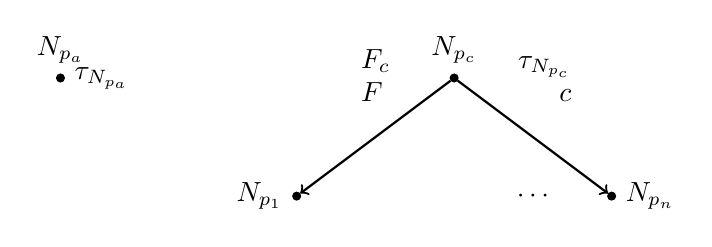
\begin{tikzpicture}[yscale=-1,
place/.style={circle,draw=black, fill=black, inner sep=0pt, 
              minimum size=1mm}]

 \node[place] (1st) at (1, 0) [label=above: $N_{p_{a}}$,
                               label=right: $\tau_{N_{p_{a}}}$] {};
	

\begin{scope}[xshift=4cm]
  \node[place] (1st) at (2, 0) [label=above: $N_{p_{c}}$,
                                label=right: 
       \begin{tabular}{l r}
         & $\tau_{N_{p_{c}}}$ \\
         & $c$\\
       \end{tabular},
       label=left:
       \begin{tabular}{l l}
         $F_c$ &\\
         $F$ &\\
       \end{tabular}] {};
  \node[place] (2nd) at (0, 1.5) [label=left: $N_{p_1}$] {};
  \node[place] (3rd) at (4, 1.5) [label=right: $N_{p_n}$]{}; 

  \node (dots) at (3,1.5) {$\cdots$};
	
  \draw[->, thick] (1st) -- (2nd);
  \draw[->, thick] (1st) -- (3rd);
\end{scope}

\end{tikzpicture}
\caption{Predicate Tree}
\label{Predicate Tree}
\end{center}   
\end{figure}

% pictures

\begin{ex}\label{ConstructPredicateTree}
Here is a part of short RFuzzy program,
\begin{center}
\begin{tabular}{l l}
$has\_tasty\_food:$  & $(Restaurant)$\\

$has\_healthy\_food:$ &  $(Restaurant)$\\

$has\_good\_service:$  & $(Restaurant)$\\

$tasty\_restaurant:$  & $(Restaurant)$\\

$good\_restaurant:$  & $(Restaurant)$\\
\end{tabular}
\end{center}
\begin{tabular}{l l l}
$tasty\_restaurant(X)$ & $\stackrel{1.0,.}{\longleftarrow} prod$ & $has\_tasty\_food(X)$\\

$good\_restaurant(X)$ & $\stackrel{0.8,.}{\longleftarrow} prod$ & $has\_healthy\_food(X), has\_good\_service(X)$ \\

\end{tabular}
\[Sim(has\_healthy\_food, has\_tasty\_food) = 0.6\]
\end{ex}

The corresponding trees for atomic predicates $has\_tasty\_food$,
$has\_healthy\_food$, $has\_good\_service$ are,
\begin{center}
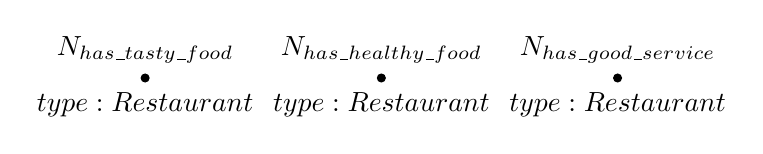
\begin{tikzpicture}[yscale=-1,
place/.style={circle,draw=black, fill=black, inner sep=0pt, 
              minimum size=1mm}]

 \node[place] (1st) at (0, 0) [label=above: $N_{has\_tasty\_food}$,
                               label=below: $type : Restaurant$] {};
	

\begin{scope}[xshift=3cm]
  \node[place] (1st) at (0, 0) [label=above: $N_{has\_healthy\_food}$,
                               label=below: $type : Restaurant$] {};
\end{scope}

\begin{scope}[xshift=6cm]
  \node[place] (1st) at (0, 0) [label=above: $N_{has\_good\_service}$,
                               label=below: $type : Restaurant$] {};
\end{scope}

\end{tikzpicture}
\end{center}   
The corresponding tree for complex predicate $tasty\_restaurant$ is,
\begin{center}
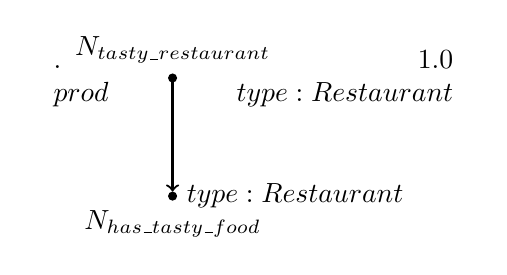
\begin{tikzpicture}[yscale=-1,
place/.style={circle,draw=black, fill=black, inner sep=0pt, 
              minimum size=1mm}]

 \node[place] (1st) at (0, 0) [label=above: $N_{tasty\_restaurant}$,
                                label=right: 
       \begin{tabular}{l r}
         & $1.0$\\
         & $type : Restaurant$ \\
       \end{tabular},
       label=left:
       \begin{tabular}{l l}
         $.$ &\\
         $prod$ &\\
       \end{tabular}] {};
  \node[place] (2nd) at (0, 1.5) [label=below: $N_{has\_tasty\_food}$,
                                  label=right: $type : Restaurant$] {};
 
  \draw[->, thick] (1st) -- (2nd);

\end{tikzpicture}
\end{center}   
The corresponding tree for complex predicate $good\_restaurant$ is,
\begin{center}
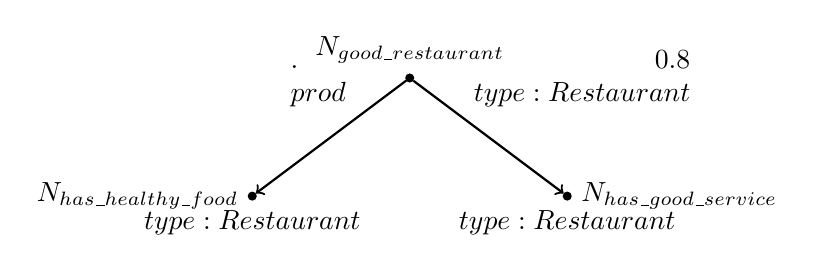
\begin{tikzpicture}[yscale=-1,
place/.style={circle,draw=black, fill=black, inner sep=0pt, 
              minimum size=1mm}]

  \node[place] (1st) at (2, 0) [label=above: $N_{good\_restaurant}$,
                                label=right: 
       \begin{tabular}{l r}
         & $0.8$\\
         & $type : Restaurant$ \\
       \end{tabular},
       label=left:
       \begin{tabular}{l l}
         $.$ &\\
         $prod$ &\\
       \end{tabular}] {};
  \node[place] (2nd) at (0, 1.5) [label=left: $N_{has\_healthy\_food}$,
                                  label=below: $type : Restaurant$] {};
  \node[place] (3rd) at (4, 1.5) [label=right: $N_{has\_good\_service}$,
                                  label=below: $type : Restaurant$]{}; 

  \draw[->, thick] (1st) -- (2nd);
  \draw[->, thick] (1st) -- (3rd);

\end{tikzpicture}
\end{center}   

If there are several rules defining a certain predicate $p$, then there are different corresponding trees for $p$, since the expanding procedure is recursive, which means, the children of $p$ node could also be defined in several other rules, then more possible trees are generated. 

\begin{prop} \textbf{Number of corresponding tree for predicate $p$}
The number of the corresponding trees for each predicate is exponential over the number of rules $n$.
\end{prop}

Let $P$ be a RFuzzy program, it has rules in the following form,
\[p() :- p_1(\vec{X})\]
\[p_1(\vec{X}) :- p_{11}(\vec{X})\]
\[p_1(\vec{X}) :- p_{12}(\vec{X})\]
\[p_{11}(\vec{X}) :- p_{111}(\vec{X})\]
\[p_{11}(\vec{X}) :- p_{112}(\vec{X})\]
\[p_{12}(\vec{X}) :- p_{121}(\vec{X})\]
\[p_{12}(\vec{X}) :- p_{122}(\vec{X})\]
\[\vdots\]
continue, for each predicate $p_{i}$, there are two rules defining it, in each rule, there is only one atom in the body.

Suppose that there is $n$ rules in $P$, and the number of trees could be generated for predicate $p$ is $2^{n/2}$, which is exponential of n. However, practically, the number of corresponding trees for certain predicate will not achieve the exponential, since the rules will be defined more reasonable, rather than the given example.

In order to retrieve the similarity between two predicates, creating all their corresponding trees is not optimal approach, considering the possible exponential explosion.  Therefore, there is a more efficient algorithm is proposed in the following sections.  


\subsubsection{Equivalence between predicate trees}
\label{sec:EquivalentTree}
In order to compare two predicate trees with different number of children, they are reconstructed with the same number of children, preserving the original semantic meaning. For this, the concept ``equivalent tree" is introduced in this section.

For each rule in $P_{new}$ that $A \stackrel{c,F_c}{\longleftarrow}F(B_1,...,B_n)$, under its interpretations, it is viewed as a function in the following form,
\[A^{\mathcal{I}} = OP (c,B_1^{\mathcal{I}},...,B_n^{\mathcal{I}})\]
where $OP=(\hat{F_c},\hat{F})$ is a pair, representing the operations over \textit{credit value} $c$, and other interpretation over atoms $B_i$ in the body of the rule. 

\begin{defin}\textbf{(Identity for complex predicate).}
\label{def:IdentityComplex}
 There exists a formula $\alpha$ under the operations of RFuzzy Program, which makes
 \begin{equation}\label{eq:equivalentFormula}
 OP(c,B_1^{\mathcal{I}},...,B_n^{\mathcal{I}},\alpha^{\mathcal{I}})=OP(c,B_1^{\mathcal{I}},...,B_n^{\mathcal{I}})
 \end{equation}
for each interpretation $\mathcal{I}$. Therefore, the formula $\alpha$ is called \textit{identity} for $OP$. The existence of $\alpha$ depends on the operation $OP$.
\end{defin}

If \textit{identity} $\alpha$ exists for some $OP$, then the rule
\begin{center}
\begin{equation}\label{eq:orginalRule}
A \stackrel{c,F_c}{\longleftarrow}F(B_1,...,B_n)
\end{equation}
\end{center}
could be rewritten as
\begin{center}
\begin{equation}\label{eq:equivalentRule}
A \stackrel{c,F_c}{\longleftarrow}F(B_1,...,B_n,\alpha,...,\alpha)
\end{equation}
\end{center}

Since the procedure of rewriting preserves the semantic equivalence, the corresponding trees of rules \ref{eq:orginalRule} and \ref{eq:equivalentRule} represent the same semantic meaning.

\begin{defin} \textbf{(Identity for atomic predicate).}
\label{def:IdentityAtomic}
For some certain $OP=(\hat{F_c},\hat{F})$, there exists a formula $\beta$ under the operations of RFuzzy Program, which makes,
\[A^{\mathcal{I}} = OP(c,A^{\mathcal{I}},\beta^{\mathcal{I}})\]
for any interpretation $\mathcal{I}$, where $c$ is a real number in the range of $[0,1]$. Therefore, $\beta$ is called identity for $OP$.
\end{defin}

\begin{comment}
We are going to show the existence of identity for any $OP=(\hat{F_c},\hat{F})$ here. In mathematical logic, there are several formal systems of \textit{Fuzzy Logic}, and most of them belong to so-called \textit{t-norm fuzzy logics} \cite{HP98}.
A t-norm abbreviated of \textit{triangular norm} is a binary algebraic operation on the interval [0, 1], which is use to generalize conjunction in t-norm fuzzy logic. A t-norm \cite{KPMRPE00} is defined as a function $\top: [0, 1]\times[0, 1]\rightarrow[0, 1]$, which satisfies the following properties:
\begin{itemize}
\item Commutativity: $\top(a, b) = \top(b, a)$
\item Monotonicity: $\top(a, b) \leq \top(c, d)$ if $a \leq c$ and $b \leq d$
\item Associativity: $\top(a, \top(b, c)) = \top(\top(a, b), c)$
\item Identity element: $\top(a, 1) = a$
\end{itemize}

T-conorm (S-norm) is dual to t-norm under the order-reversing operation which assigns 1-x to x on [0, 1]. Given a t-norm, the complementary t-conorm is defined by
\[\bot(a,b) = 1- \top(1-a,1-b)\]
A t-conorm is used to represent logical disjunction in t-norm fuzzy logic. It satisfies the following conditions, which can be used for an equivalent axiomatic definition of t-conorm independently of t-norm:
\begin{itemize}
\item Commutativity: $\bot(a, b) = \bot(b, a)$
\item Monotonicity: $\bot(a, b) \leq \bot(c, d)$ if $a \leq c$ and $b \leq d$
\item Associativity: $\bot(a, \bot(b, c)) = \bot(\bot(a, b), c)$
\item Identity element: $\bot(a, 0) = a$
\end{itemize}

$\hat{F_c}$ and $\hat{F}$  are the truth functions of many-valued connectives $F_c$ and $F$ respectively. They are defined by t-norm or t-conorm. It implies that for any $\hat{F_c}$ or $\hat{F}$, there exists an identity, since a t-norm and a t-conorm has $1$ and $0$ as their identities respectively. Taking Lukasiewicz logic \cite{L20} as an instance, which is one of t-norm fuzzy logics originally defined in the early 20th-century by Jan Lukasiewicz. The connectives and their functions are shown below.
\begin{itemize}
\item Implication: $F_{\rightarrow}(x,y) = min\{1,1-x+y\}$
\item Equivalence: $F_{\leftrightarrow}(x,y) = 1-\lvert x-y \rvert$
\item Negation:  $F_{\neg}(x) = 1-x$
\item Weak Conjunction: $F_{\wedge}(x,y)=min\{x,y\}$
\item Weak Disjunction:  $F_{\vee}(x,y)=max\{x,y\}$
\item Strong Conjunction: $F_{\otimes}(x,y)=max\{0,x+y-1\}$
\item Strong Disjunction:   $F_{\oplus}(x,y)=min\{1,x+y\}$
\end{itemize}
The connectives defined by t-norm are Equivalence, Weak Conjunction, Strong Disjunction, which have $1$ as their identities. Implication, Weak Disjunction, Strong Conjunction are defined by t-conorm and $0$ is the identity.

For example, $F_{\rightarrow}(x,y) = F_{\rightarrow}(F_{\rightarrow}(x,y),1)$, if we use $F_{\rightarrow}$ to represent implication with arbitrary arguments, then $F_{\rightarrow}(x,y) = F_{\rightarrow}(x,y,1)$, which satisfies formula \ref{eq:equivalentFormula} in definition \ref{def:IdentityComplex}.

\end{comment}




\subsubsection{Reconstructing predicate trees with equivalence}
\label{sec:ReConstruct}
In this section, the approach of constructing predicates tree with equivalence is displayed, which is used for expanding two comparing nodes with the same structure in the algorithm introduced in section \ref{sec:Algorithm}.

%\begin{center}
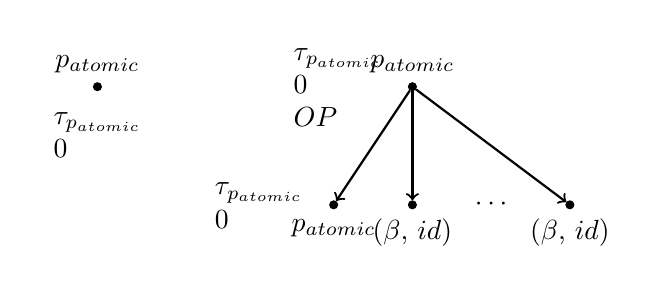
\begin{tikzpicture}[yscale=-1,
place/.style={circle,draw=black, fill=black, inner sep=0pt, 
              minimum size=1mm}]

	\node[place] (1st) at (1, 0) [label=above: $p_{atomic}$,
                                      label=below:
            \begin{tabular}{l}
              $\tau_{p_{atomic}}$\\
              $0$\\
            \end{tabular}] {};

\begin{scope}[xshift=4cm]
  \node[place] (1st) at (1, 0) [label=above: $p_{atomic}$,
                                label=left: 
             \begin{tabular}{l}
              $\tau_{p_{atomic}}$\\
              $0$\\
              $OP$\\ 
             \end{tabular}
] {};
	\node[place] (2nd) at (0, 1.5) [label=below: $p_{atomic}$,
                                        label=left: 
             \begin{tabular}{l}
              $\tau_{p_{atomic}}$ \\
              $0$ \\
             \end{tabular}
]{};
        \node[place] (3rd) at (1, 1.5) [label=below: {($\beta$, $id$)}] {};
	\node[place] (4rd) at (3, 1.5) [label=below: {($\beta$, $id$)}] {}; 

	\node (dots) at (2,1.5) {$\cdots$};
	
	\draw[->, thick] (1st) -- (2nd);
	\draw[->, thick] (1st) -- (3rd);
        \draw[->, thick] (1st) -- (4rd);
\end{scope}


\end{tikzpicture}
\end{center}   

\begin{itemize}
 \item \textit{Atomic predicate}

Suppose that $p_a$ is a \textit{atomic predicate}. Its type is $\tau$. The identity for some $OP$ associated with $p_a$ is $\beta$. 

The corresponding tree of it is a node $N_{p_a}$ with information, which are $\tau$ of $p_a$ and a number $0$, indicating that $p_a$ is atomic predicate. There are no branches for the node $N_{p_a}$. 

With the equivalence extension, the corresponding tree is presented in figure \ref{fig:APT}. The root is a node $N_{p_a}$ with information, which are the \textit{type} of $p_a$ $\tau$, the operation $OP$ and atomic mark $0$. The branches are a node $N'_{p_a}$ and several nodes $N_{\beta}$.  $N'_{p_a}$ carries information $\tau$, which is $p_a$�s type and atomic mark $0$. $N_{\beta}$ carries information of identity $\beta$ and identity mark $id$, the number of such nodes depends on two comparing predicates.

% pictures
\begin{figure}[h!]
\begin{center}
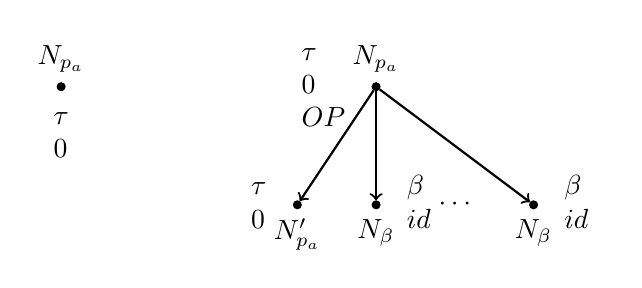
\begin{tikzpicture}[yscale=-1,
place/.style={circle,draw=black, fill=black, inner sep=0pt, 
              minimum size=1mm}]

	\node[place] (1st) at (1, 0) [label=above: $N_{p_a}$,
                                      label=below:
            \begin{tabular}{l}
              $\tau$\\
              $0$\\
            \end{tabular}] {};

\begin{scope}[xshift=4cm]
  \node[place] (1st) at (1, 0) [label=above: $N_{p_a}$,
                                label=left: 
             \begin{tabular}{l}
               $\tau$\\
               $0$\\
               $OP$\\
             \end{tabular}
] {};
	\node[place] (2nd) at (0, 1.5) [label=below: $N'_{p_a}$,
                                        label=left: 
             \begin{tabular}{l}
              $\tau$ \\
              $0$ \\
             \end{tabular}
]{};
        \node[place] (3rd) at (1, 1.5) [label=below: $N_{\beta}$,
        							  label=right: 
             \begin{tabular}{l}
              $\beta$ \\
              $id$ \\
             \end{tabular}        
        ] {};
	\node[place] (4rd) at (3, 1.5) [label=below: $N_{\beta}$,
							  label=right: 
             \begin{tabular}{l}
              $\beta$ \\
              $id$ \\
             \end{tabular}
	] {}; 

	\node (dots) at (2,1.5) {$\cdots$};
	
	\draw[->, thick] (1st) -- (2nd);
	\draw[->, thick] (1st) -- (3rd);
         \draw[->, thick] (1st) -- (4rd);
\end{scope}


\end{tikzpicture}
\end{center}   
\caption{Atomic predicate tree with equivalence}
\label{fig:APT}
\end{figure}

 \item \textit{Complex predicate}

For \textit{complex predicate}, there would be at least one rule defining it as,
\[p_c(\vec{t}) \stackrel{c,F_c}{\longleftarrow}F(p_1(\vec{t_1}),...,p_n(\vec{t_n}))\]
and for $OP=(\hat{F_c},\hat{F})$, there exists an identity $\alpha$.  $\tau$, and $\tau_{i}$ are represented types of $p_c$ and $p_{i}$ respectively.

The corresponding tree for $p_c$ is

% pciture
\begin{center}
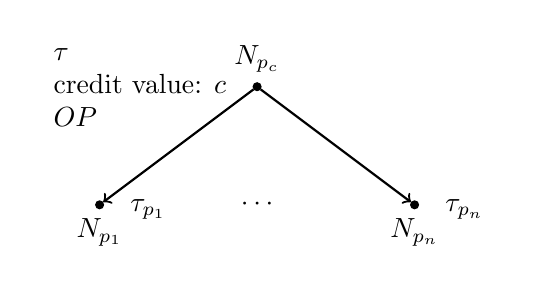
\begin{tikzpicture}[yscale=-1,
place/.style={circle,draw=black, fill=black, inner sep=0pt, 
              minimum size=1mm}]

  \node[place] (1st) at (2, 0) [label=above: $N_{p_c}$,
                                label=left: 
             \begin{tabular}{l}
               $\tau$\\
               credit value: $c$\\
               $OP$\\
             \end{tabular}
] {};
	\node[place] (2nd) at (0, 1.5) [label=below: $N_{p_1}$,
							  label=right: 
             \begin{tabular}{l}
            $\tau_{p_1}$\\
             \end{tabular}
	] {};
        \node[place] (3rd) at (4, 1.5) [label=below: $N_{p_n}$,
        							label=right: 
             \begin{tabular}{l}
             $\tau_{p_n}$ \\
             \end{tabular}        
        ] {}; 
	
	\node (dots) at (2,1.5) {$\cdots$};
	
	\draw[->, thick] (1st) -- (2nd);
	\draw[->, thick] (1st) -- (3rd);
        

\end{tikzpicture}
\end{center}   

where $N_{p_c}$ is the root with information which are $\tau$, $OP$ and credit value $c$. $N_{p_i}$s are the branches carrying their \textit{types} as information.

With the equivalence extension, the tree is 

% pictures
\begin{center}
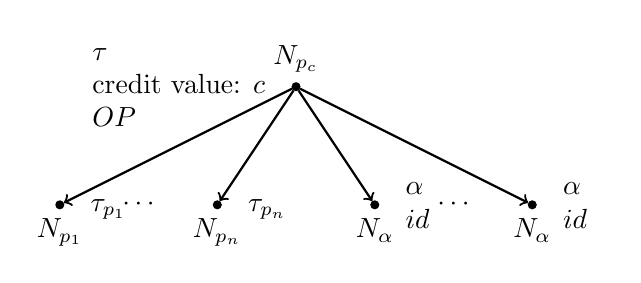
\begin{tikzpicture}[yscale=-1,
place/.style={circle,draw=black, fill=black, inner sep=0pt, 
              minimum size=1mm}]

  \node[place] (1st) at (3, 0) [label=above: $N_{p_c}$,
                                label=left: 
             \begin{tabular}{l}
               $\tau$\\
               credit value: $c$\\
               $OP$\\
             \end{tabular}
] {};
	\node[place] (2nd) at (0, 1.5) [label=below: $N_{p_1}$,
							label=right: 
             \begin{tabular}{l}
            $\tau_{p_1}$\\
             \end{tabular}
	] {};
	\node[place] (3rd) at (2, 1.5) [label=below: $N_{p_n}$,
							  label=right: 
             \begin{tabular}{l}
            $\tau_{p_n}$\\
             \end{tabular}
	] {}; 
        \node[place] (4rd) at (4, 1.5) [label=below: $N_{\alpha}$,
        						  label=right: 
             \begin{tabular}{l}
            $\alpha$\\
            $id$\\
             \end{tabular}
        ] {}; 
        \node[place] (5rd) at (6, 1.5) [label=below: $N_{\alpha}$,
        						  label=right: 
             \begin{tabular}{l}
            $\alpha$\\
            $id$
             \end{tabular}
	] {}; 

	\node (dots) at (1,1.5) {$\cdots$};
        \node (dots) at (5,1.5) {$\cdots$};
	
	\draw[->, thick] (1st) -- (2nd);
	\draw[->, thick] (1st) -- (3rd);
        \draw[->, thick] (1st) -- (4rd);
        \draw[->, thick] (1st) -- (5rd);
\end{tikzpicture}
\end{center}   
 $N_{p_c}$ is the root with information which are $\tau$, $OP$ and credit value $c$. $N_{p_i}$s are the branches with their \textit{types} as information, and several nodes $N_{\alpha}$ carrying information of identities $\alpha$ with identity mark $id$ are added as extra branches depending on two comparing predicates.
\end{itemize}

\begin{ex}
Continuation of the example \ref{ConstructPredicateTree}, reconstruct predicate trees with equivalence.

\begin{center}
\begin{tabular}{l l}
$has\_tasty\_food:$  & $(Restaurant)$\\

$has\_healthy\_food:$ &  $(Restaurant)$\\

$has\_good\_service:$  & $(Restaurant)$\\

$tasty\_restaurant:$  & $(Restaurant)$\\

$good\_restaurant:$  & $(Restaurant)$\\
\end{tabular}
\end{center}
\begin{tabular}{l l l}
$tasty\_restaurant(X)$ & $\stackrel{1.0,.}{\longleftarrow} prod$ & $has\_tasty\_food(X)$\\

$good\_restaurant(X)$ & $\stackrel{0.8,.}{\longleftarrow} prod$ & $has\_healthy\_food(X), has\_good\_service(X)$ \\
\end{tabular}

The predicate tree for \textit{has\_tasty\_food} is represented in figure \ref{fig:ex1}.
\begin{figure}[h!]
\begin{center}
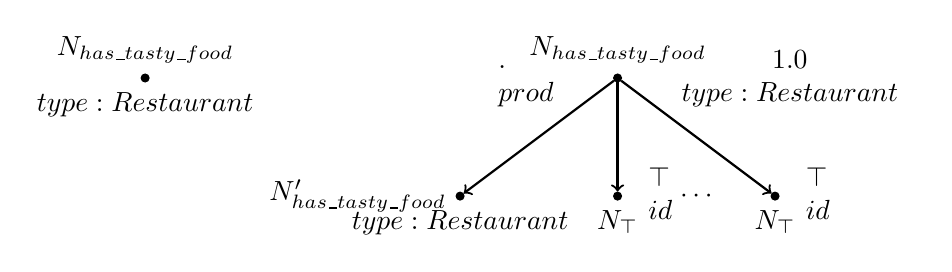
\begin{tikzpicture}[yscale=-1,
place/.style={circle,draw=black, fill=black, inner sep=0pt, 
              minimum size=1mm}]

 \node[place] (1st) at (0, 0) [label=above: $N_{has\_tasty\_food}$,
                               label=below: $type : Restaurant$] {};
	

\begin{scope}[xshift=4cm]
  \node[place] (1st) at (2, 0) [label=above: $N_{has\_tasty\_food}$,
                                label=right: 
       \begin{tabular}{l c}
         & $1.0$\\
         & $type : Restaurant$ \\
       \end{tabular},
       label=left:
       \begin{tabular}{l l}
         $.$ &\\
         $prod$ &\\
       \end{tabular}] {};
  \node[place] (2nd) at (0, 1.5) [label=left: $N'_{has\_tasty\_food}$,
                                  label=below: $type : Restaurant$] {};
  \node[place] (3rd) at (2, 1.5) [label=below: $N_{\top}$,
  						  label=right: 
             \begin{tabular}{l}
            $\top$\\
            $id$\\
             \end{tabular}
	]{}; 

  \node[place] (4th) at (4, 1.5) [label=below: $N_{\top}$,
    						  label=right: 
             \begin{tabular}{l}
            $\top$\\
            $id$\\
             \end{tabular}
  ]{};

  \node (dots) at (3,1.5) {$\cdots$};

  \draw[->, thick] (1st) -- (2nd);
  \draw[->, thick] (1st) -- (3rd);
  \draw[->, thick] (1st) -- (4th);
\end{scope}

\end{tikzpicture}
\end{center}   
\caption{two equivalent predicate trees for has\_tasty\_food}
\label{fig:ex1}
\end{figure}

The predicate tree for \textit{tasty\_restaurant} is represented in figure \ref{fig:ex2.1}, and \ref{fig:ex2.2} which is extended with equivalence.
\begin{figure}[h!]
\begin{center}
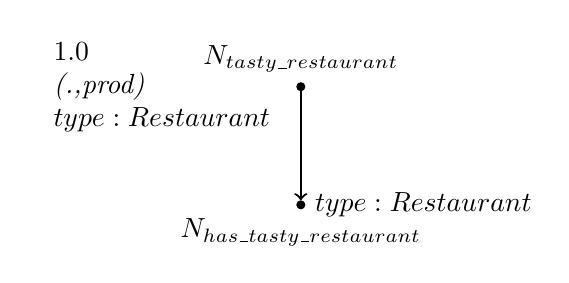
\begin{tikzpicture}[yscale=-1,
place/.style={circle,draw=black, fill=black, inner sep=0pt, 
              minimum size=1mm}]

\node[place] (1st) at (0, 0) [label=above: $N_{tasty\_restaurant}$,
                              label=left: 
             \begin{tabular}{l}
               $1.0$\\
               \textit{(.,prod)}\\
               $type : Restaurant$\\
             \end{tabular}
] {};
\node[place] (2nd) at (0, 1.5) [label=below:  $N_{has\_tasty\_restaurant}$,
label=right: 
$type : Restaurant$] {};
        
	\draw[->, thick] (1st) -- (2nd);
	
\end{tikzpicture}
\end{center}
\caption{predicate tree for tasty\_restaurant}
\label{fig:ex2.1}   
\end{figure}
\newpage
\begin{figure}
\begin{center}
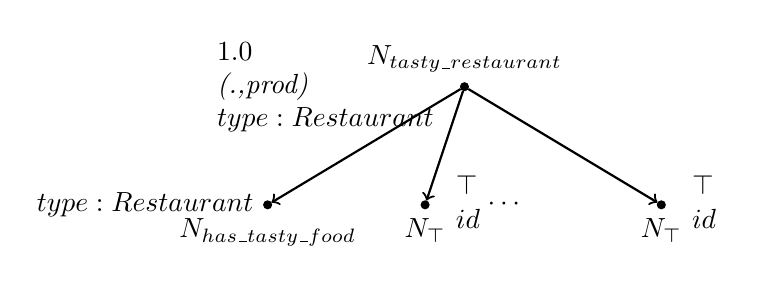
\begin{tikzpicture}[yscale=-1,
place/.style={circle,draw=black, fill=black, inner sep=0pt, 
              minimum size=1mm}]

  \node[place] (1st) at (2.5, 0) [label=above: $N_{tasty\_restaurant}$,
                                label=left: 
             \begin{tabular}{l}
               $1.0$\\
               \textit{(.,prod)}\\
               $type : Restaurant$\\
             \end{tabular}
] {};
	\node[place] (2nd) at (0, 1.5) [label=below: $N_{has\_tasty\_food}$, 
        label=left: $type : Restaurant$] {};
        \node[place] (3rd) at (2, 1.5) [label=below: $N_{\top}$,
          						  label=right: 
             \begin{tabular}{l}
            $\top$\\
            $id$\\
             \end{tabular}
             ] {}; 
        \node[place] (4rd) at (5, 1.5) [label=below: $N_{\top}$,
          						  label=right: 
             \begin{tabular}{l}
            $\top$\\
            $id$\\
             \end{tabular}
             ] {}; 

        \node (dots) at (3,1.5) {$\cdots$};
	
	\draw[->, thick] (1st) -- (2nd);
        \draw[->, thick] (1st) -- (3rd);
        \draw[->, thick] (1st) -- (4rd);
\end{tikzpicture}
\end{center}   
\caption{predicate tree for tasty\_restaurant with equivalence extension}
\label{fig:ex2.2}
\end{figure}
\end{ex}


\subsection{Algorithm for similarity}
% Comparing similarity between two trees-------the algorithm
\label{sec:Algorithm}
Let $p_a$ and $p_b$ be arbitrary predicates in RFuzzy Program $P$.
The similarity value is represented as a pair $(level,sim\_degree) \in \mathbb{Z}/\mathbb{Z^+} \times \{[0,1],u\}$, where $level$ is a nonpositive integer representing the level of expansion of the corresponding tree, and $sim\_degree$ is a real number ranging from $0$ to $1$ representing the similarity degree between two predicates or a mark $u$ to represent that the similarity degree has not been defined.

($\mathbb{Z}/\mathbb{Z^+} \times [0,1]$, $\leq$) is a partial set. Suppose that $r_1$, $r_2$ are two real numbers in $[0,1]$, where $r_1 \leq r_2$. We have a partial order such as,
\[\dots \leq(-3,0) \leq (-3,r_1) \leq (-3,r_2) \leq (-3,1) \leq \]
\[\dots \leq (0,0) \leq (0,r_1) \leq (0,r_2) \leq (0,1)\]
Therefore, arbitrary two pairs $(l_1,v_1)$, $(l_2,v_2)$ are in $\mathbb{Z}/\mathbb{Z^+} \times [0,1]$, $(l_1,v_1) \leq (l_2,v_2)$ \textbf{iff} $l_1 < l_2$ \textit{or} $l_1 = l_2$ and $v_1 \leq v_2$.
 
Let $p_a$ and $p_b$ be predicates with types $\tau_{p_a}$ and $\tau_{p_b}$, respectively. The similarity between them is defined in the following approach.
\begin{itemize}
 \item \textit{atomic predicate VS atomic predicate} 

   $p_a$ and $p_b$ are \textit{atomic predicates}, which are represented to be isolated nodes with information $\tau_{p_a}$ and $\tau_{p_b}$ as \textit{type} of $p_a$ and $p_b$, respectively. If $\tau_{p_a}=\tau_{p_b}$, in the sense that $p_a$ and $p_b$ have the same \textit{type}, then similarity degree between $p_a$ and $p_b$ should be defined directly as a real number in $[0,1]$ in RFuzzy program $P$ as $sim\_degree$. Then the similarity value is $Sim(p_a,p_b)=(l,sim\_degree)$, where $l$ is the level of expansion. Once no such information found in RFuzzy program $P$, return $(-\infty,0)$ as default similarity value, which means the similarity can not be found even though the predicates could be expanded until infinite level.

% picture
\begin{figure}[h!]
\begin{center}
\begin{tikzpicture}[yscale=-1,
place/.style={circle,draw=black, fill=black, inner sep=0pt, 
              minimum size=1mm}]

  \node[place] (1st) at (1, 0) [label=above: $p_a$,
                                label=left: $\tau_{p_a}$] {};
\begin{scope}[xshift=4cm]
  \node[place] (1st) at (1, 0) [label=above: $p_b$,
                                label=right: $\tau_{p_b}$] {};
\end{scope}

);
\end{tikzpicture}
\end{center}
\caption{Comparison between two atomic predicates}   
\label{fig:SimAA}
\end{figure}
 \item \textit{atomic predicate VS complex predicate}

   $p_a$ is an atomic predicate, and $p_b$ is a complex predicate.
   Then, $p_a$ is represented as an isolated node with information which are $\tau_{p_a}$ and $0$ as  atomic  mark. While, $p_b$ is represented as an isolated node with information $\tau_{p_b}$. The similarity between them is achieved by following,

   \begin{enumerate}
    \item If $\tau_{p_a} \neq \tau_{p_b}$ then $Sim(p_a,p_b) = (-\infty,0)$

    \item If $\tau_{p_a} = \tau_{p_b}$, then search for defined $sim\_degree$ in RFuzzy program, which is a real number in $[0,1]$. If there exists, then return the similarity value as $(l,sim\_degree)$, where $l$ is the level of expansion which $p_a$ and $p_b$ are on. 
 
    \item If $\tau_{p_a} = \tau_{p_b}$ and there doesn't exist the defined similarity in RFuzzy program, then two steps are taken afterwards,
    \begin{itemize}
     \item Return a middle result $Sim(p_a,p_b)=(l,u)$, where $l$ is the level of expansion which $p_a$ and $p_b$ are on and $u$ represents the similarity degree is undefined.
     \item Expand $p_a$ and $p_b$ in the following way.
    $p_b$ is expanded according to its rule
    \[p_b(\vec{t}) \stackrel{c,F_c}{\longleftarrow}F(p_1(\vec{t_1}),...,p_n(\vec{t_n}))\]
    $N_{p_b}$ is the root with information $INFO_{p_b} = \{c,OP=(\hat{F_c},\hat{F}),\tau_{p_b}\}$. Its branches are nodes $N_{p_1}$, ..., $N_{p_n}$ with \textit{type} $\tau_{p_1}$, $\dots$, $\tau_{p_n}$ of $p_1$, $\dots$, $p_n$ respectively.
    % picture
    $p_a$ is expanded according to $OP$ in $INFO_{p_b}$, then $N_{p_a}$ is the root with $INFO_{p_a} = \{c',OP=(\hat{F_c},\hat{F}),\tau_{p_a}\}$. Its branches are nodes $N'_{p_a}$, $N_{\beta}$, ...,$N_{\beta}$. The number of children of $N_{p_a}$ is $n$, which is the same as $N_{p_b}$.
   \end{itemize}

\begin{figure}[h!]
\begin{center}
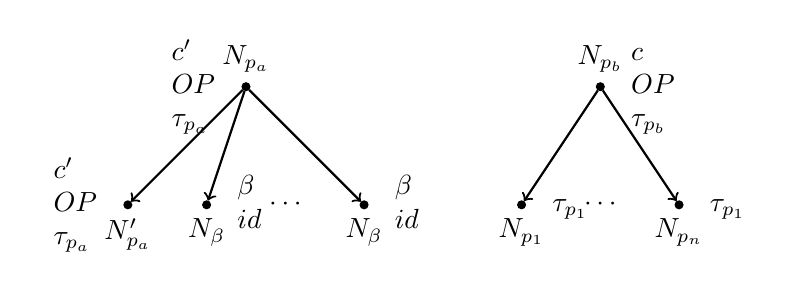
\begin{tikzpicture}[yscale=-1,
place/.style={circle,draw=black, fill=black, inner sep=0pt, 
              minimum size=1mm}]

  \node[place] (1st) at (1.5, 0) [label=above: $N_{p_a}$,
                                  label=left: 
     \begin{tabular}{l}
        $c'$\\
        $OP$\\
        $\tau_{p_a}$\\  
     \end{tabular}
] {};
  \node[place] (2nd) at (0, 1.5) [label=below: $N'_{p_a}$,
                                  label=left:
     \begin{tabular}{l}
        $c'$\\
        $OP$\\
        $\tau_{p_a}$\\  
     \end{tabular}
]{};
  \node[place] (3rd) at (1, 1.5) [label=below: $N_{\beta}$, 
    label=right: 
             \begin{tabular}{l}
            $\beta$\\
            $id$\\
             \end{tabular}
	] {}; 
  \node[place] (4th) at (3, 1.5) [label=below: $N_{\beta}$,
    label=right: 
             \begin{tabular}{l}
            $\beta$\\
            $id$\\
             \end{tabular}
             ] {}; 

  \node (dots) at (2,1.5) {$\cdots$};
	
  \draw[->, thick] (1st) -- (2nd);
  \draw[->, thick] (1st) -- (3rd);
  \draw[->, thick] (1st) -- (4th);

\begin{scope}[xshift=5cm]
  \node[place] (1st) at (1, 0) [label=above: $N_{p_b}$,
                                label=right: 
     \begin{tabular}{l}
        $c$\\
        $OP$\\
        $\tau_{p_b}$\\
     \end{tabular}
] {};
  \node[place] (2nd) at (0, 1.5) [label=below: $N_{p_1}$, 
    label=right: 
             \begin{tabular}{l}
            $\tau_{p_1}$\\
             \end{tabular}
             ] {};
  \node[place] (3rd) at (2, 1.5) [label=below: $N_{p_n}$, 
  label=right: 
             \begin{tabular}{l}
            $\tau_{p_1}$\\
             \end{tabular}
             ] {}; 

  \node (dots) at (1,1.5) {$\cdots$};
	
  \draw[->, thick] (1st) -- (2nd);
  \draw[->, thick] (1st) -- (3rd);
\end{scope}

);
\end{tikzpicture}
\end{center}
\caption{Comparison between atomic and complex predicates}
\label{fig:SimAC}
\end{figure}   % Picture

   \end{enumerate}
 
 \item \textit{complex predicate VS complex predicate}

   $p_a$ and $p_b$ are complex predicates with $\tau_{p_a}$ and $\tau_{p_b}$ as \textit{type}, respectively. If $p_a$ and $p_b$ are of the different \textit{types}, that is, $\tau_{p_a} \neq \tau_{p_b}$, then $Sim(p_a, p_b)=(-\infty,0)$ will be returned, otherwise, the expanding procedure will be carried on according to the fuzzy rules.
    $p_a$ is defined by rule
    \[p_a(\vec{t}) \stackrel{c^a,F_c^a}{\longleftarrow}F^a(p_1^a(\vec{t_1^a}),...,p_n^a(\vec{t_n^a}))\]
    with $OP_a=(F_c^a,F^a)$
    and $p_b$ is defined by rule
    \[p_b(\vec{t}) \stackrel{c^b,F_c^b}{\longleftarrow}F^b(p_1^b(\vec{t_1^b}),...,p_m^b(\vec{t_m^b}))\]
    with $OP_b=(F_c^b,F^b)$. There are two cases of $p_a$ and $p_b$ expansion.
   \begin{enumerate}
    \item $p_a$ and $p_b$ are defined by the different $OP$
     
     If $OP_a \neq OP_b$, which is, $F_c^a \neq F_c^b$ or $F^a \neq F^b$, then return $0$ as similarity degree, and $Sim(p_a, p_b)=(-\infty,0)$. 
   
    \item $p_a$ and $p_b$ are defined by the same $OP$
   
     If $OP_a=OP_b$, which is $F_c^a=F_c^b$ and $F^a=F^b$, then
     same two steps are taken here,
    \begin{itemize}
     \item Return middle result $Sim(p_a,p_b)=(l,u)$
     \item Continue the identity formalization, after which, $p_a$ and $p_b$ have corresponding trees with the same construction, where the roots are of the same type, the same $OP$, and have the same number of children. The comparing procedure of their children is recursively defined.
\end{itemize}
   \end{enumerate}

\begin{figure}[h!]
\begin{center}
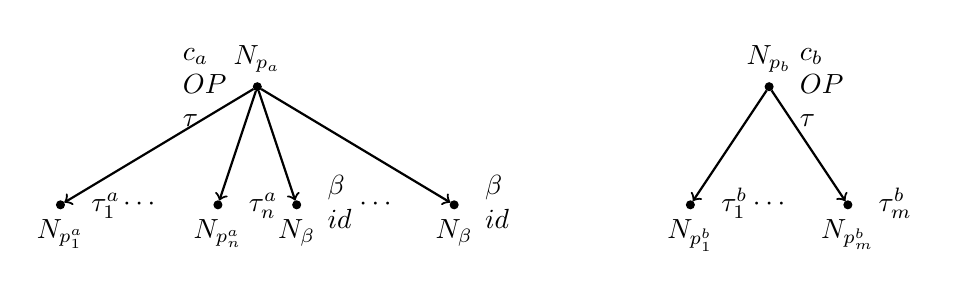
\begin{tikzpicture}[yscale=-1,
place/.style={circle,draw=black, fill=black, inner sep=0pt, 
              minimum size=1mm}]

  \node[place] (1st) at (2.5, 0) [label=above: $N_{p_a}$,
                                label=left: 
    \begin{tabular}{l}
      $c_a$\\
      $OP$\\
      $\tau$\\ 
    \end{tabular}
] {};
  \node[place] (2nd) at (0, 1.5) [label=below:  $N_{p_1^a}$,
  	label=right:
    		\begin{tabular}{l}
    			 $\tau_1^a$\\ 
   		 \end{tabular} ] {};
  \node[place] (3rd) at (2, 1.5) [label=below:   $N_{p_n^a}$,    
  	label=right:   
   		\begin{tabular}{l}
       			$\tau_n^a$\\ 
    		\end{tabular}] {}; 
  \node[place] (4th) at (3, 1.5) [label=below:  $N_{\beta}$,
  	label=right:
  	\begin{tabular}{l}
     		$\beta$\\
     		$id$\\ 
    	\end{tabular}] {}; 
  \node[place] (5th) at (5, 1.5) [label=below:  $N_{\beta}$,
  label=right:
  	\begin{tabular}{l}
     		$\beta$\\
     		$id$\\ 
    	\end{tabular}] {}; 
  
  \node (dots) at (1,1.5) {$\cdots$};
  \node (dots) at (4,1.5) {$\cdots$};
	
  \draw[->, thick] (1st) -- (2nd);
  \draw[->, thick] (1st) -- (3rd);
  \draw[->, thick] (1st) -- (4th);
  \draw[->, thick] (1st) -- (5th);


\begin{scope}[xshift=8cm]
  \node[place] (1st) at (1, 0) [label=above: $N_{p_b}$,
                                label=right: 
       \begin{tabular}{l}
         $c_b$\\
         $OP$\\
         $\tau$\\
       \end{tabular}
] {};
  \node[place] (2nd) at (0, 1.5) [label=below:  $N_{p_1^b}$,
  label=right:
  \begin{tabular}{l}
     $\tau_1^b$\\ 
    \end{tabular}]{};
  \node[place] (3rd) at (2, 1.5) [label=below:  $N_{p_m^b}$,
  label=right:
  \begin{tabular}{l}
     $\tau_m^b$\\ 
    \end{tabular}] {}; 

  \node (dots) at (1,1.5) {$\cdots$};
	
  \draw[->, thick] (1st) -- (2nd);
  \draw[->, thick] (1st) -- (3rd);
\end{scope}

);
\end{tikzpicture}
\end{center}
\caption{Comparison between two complex predicates} 
\label{fig:SimCC}
\end{figure}
%picture

\end{itemize}

For each expansion, the middle result which is the similarity value before next expansion and comparison, must be returned to filter some pairs of corresponding trees to reduce unnecessary expansion or comparison. The middle result of one level is formalized as follow.

Suppose that $p_a$ and $p_b$ are on level $l$ in their own trees, and are satisfied expanding requirements with $n$ children for each.
After combination of their children, $n$ optimal $Sim(p_i^a,p_j^b)$ are returned and composed as a \textit{middle set} $M_s$. The possible values in $M_s$ are $(-\infty,0)$, $(l-1,sim\_degree)$, $(l-1,u)$, where $sim\_degree \in [0,1]$. There is one subset of $M_s$, called \textit{decision middle set}, defined as,
\begin{equation}\label{eq:DecisionMiddleSet}
M_{ds}=\{(level,degree)| level \neq -\infty, degree \neq u\}
\end{equation}
The \textit{middle result} is $M_r = (l-1,M_v)$, where $M_v$ is defined as, 
\begin{equation}\label{eq:MiddleResult}
M_v=\frac{\sum_{i=1}^{m} v_i+1-\lvert c^a-c^b\rvert}{n+1}
\end{equation}
where $m$ is the cardinality of $M_{ds}$, $v_i$ is an element in $M_{ds}$. 

There are three points to be emphasized.
\begin{enumerate}
\item Similarity between identity and an arbitrary predicate

	The purpose of introducing identity $\alpha$ for an operation $OP=(\hat{F_c},\hat{F})$ is to build two predicate tree in the same structure, where two predicate trees have the identical $OP$ and the same number of children. The procedure of reconstructing predicate tree with equivalence preserves the original semantics. When comparing identity $\alpha$ and an arbitrary predicate $p$, the similarity between them is defined as $Sim(\alpha, p) = (l, v)$, where $l$ is the level the identity is on, and $v$ is an arbitrary value in $[0,1]$. The value $v$ will not affect the decision of choosing the optimal combination. The reason is shown in next point. 
	 
\item The property of Middle Result

	The \textit{middle result} is an element in $\mathbb{Z}/\mathbb{Z^+} \times [0,1]$, which is a partial order. The combination with precedent \textit{middle result} is chosen to be optimal combination, which is used to the next expansion. There are three questions are answered here. 
\begin{enumerate}	
\item Is $v$ in $Sim(\alpha,p)=(l,v)$ will affect the decision of choosing the optimal combination ? 
\item Why does precedent \textit{middle result} decide the optimal combination ?
\item What is the meaning of  $1- \lvert c^a - c^b  \rvert$ ?
\end{enumerate}
 	\begin{itemize}
	
	\item The affect of $Sim(\alpha, p)=(l,v)$
		
		 Suppose that obtaining similarity between $p_a$ and $p_b$ needs expansion. $p_a$, $p_b$ has $x$ and $y$ children respectively, and $x>y$. By building equivalent predicate tree for $p_b$, $x-y$ identities $\alpha$ are added as extra children of $p_b$. In any combinations of $x$ children in $p_a$ and $x$ children in $p_b$,  the number of $Sim(\alpha, p)$ is the same, which is $x-y$. According to formula \ref{eq:MiddleResult}, $M_v$ is monotonic increase on $v_i$. So the value of $v$ in $Sim(\alpha, p)=(l,v)$ will not affect on choosing an optimal combination.
		 
	\item The optimal combination
	
		In formula \ref{eq:DecisionMiddleSet}, $(-\infty,0)$ and $(l-1,u)$ are excluded from \textit{decision middle set} $M_{ds}$. The cardinality $m$ of $M_{ds}$ will affect the \textit{middle result} $M_r=(l-1,M_v)$, since $M_v$ is monotonic increase on $m$.  $(-\infty,0)$ means two predicates are not comparable and $(l-1,u)$ means similarity of two predicates are not defined in level $l-1$. Thus, the combination with more comparable pairs of predicates and more pairs of predicates with defined similarity has precedent \textit{middle result}.
		
	\item similarity between credit value
	
		Credit value $c^a$ and $c^b$ are the trust degrees of fuzzy rules within head $p_a$ and $p_b$, respectively. They are values in unit interval $[0,1]$. We define the distance between 
$c^a$ and $c^b$ by $1-norm$, which is $\lvert c^a-c^b \rvert$. The similarity between them is  $1- \lvert c^a - c^b  \rvert$. $c^a$ and $c^b$ are considered as a special pair of combinations, whose similarity is counted into the middle result of similarity between $p_a$ and $p_b$.  
	\end{itemize}
	
\item The termination of algorithm
	
	For any comparing pair $(p_i^a,p_j^b)$ from children of $p_a$ and $p_b$, if $Sim(p_i^a,p_j^b)=(l-1,u)$, it means that $p_i^a$ and $p_j^b$ have the same type but the similarity degree have not been defined directly in the RFuzzy program, and it could be reached by expanding them according to certain rules. The expanding procedure could be continued until both comparing predicates are atomic, which makes the algorithm terminate.
\end{enumerate} 


The algorithm terminates \textbf{iff} the comparing trees of predicates are \textit{completely built}.

\begin{defin} \textbf{Completely Built}.
The two comparing predicates are represented as trees, and expanded and valued in synchronization with each other until no comparing value $(level,u)$ is returned. Then the comparing trees are \textit {completely built}. The \textbf{similarity degree} is calculated from leaves to root by the definition of \textit{middle value}, and the \textbf{level} is the lowest level of the comparing trees.
\end{defin}

\begin{ex}

Here is a short RFuzzy program from the example \ref{ConstructPredicateTree},
\begin{center}
\begin{tabular}{l l}
$has\_tasty\_food:$  & $(Restaurant)$\\

$has\_healthy\_food:$ &  $(Restaurant)$\\

$has\_good\_service:$  & $(Restaurant)$\\

$tasty\_restaurant:$  & $(Restaurant)$\\

$good\_restaurant:$  & $(Restaurant)$\\
\end{tabular}
\end{center}
\begin{tabular}{l l l}
$tasty\_restaurant(X)$ & $\stackrel{1.0,.}{\longleftarrow} prod$ & $has\_tasty\_food(X)$\\

$good\_restaurant(X)$ & $\stackrel{0.8,.}{\longleftarrow} prod$ & $has\_healthy\_food(X), has\_good\_service(X)$ \\

\end{tabular}
\[Sim(has\_healthy\_food, has\_tasty\_food) = 0.6\]

\end{ex}
The set of \textit{Atomic predicates} is $AP= \{has\_tasty\_food, has\_healthy\_food, \linebreak[4]has\_good\_service\}$, and the set of \textit{complex predicates} is $CP= \{tasty\_restaurant,  \linebreak[4]good\_restaurant\}$. They have the same \textit{type} `Restaurant'. There are two tasks as examples for gaining the similarity, one is between  $tasty\_restaurant$ and $has\_tasty\_restaurant$, and the other is between $tasty\_restaurant$ and  \linebreak[4]$good\_restaurant$.

\begin{itemize}
 \item $Sim(tasty\_restaurant,has\_tasty\_food)$

Since $tasty\_restaurant \in CP$, and $has\_tasty\_food \in AP$, the procedure of obtaining similarity follows the case ``atomic predicate VS complex predicate''.
In an abbreviation, $tr$ is represented as $tasty\_restaurant$, $htf$ is for $has\_tasty\_food$, $R$ means `Restaurant'.
\newpage
\begin{figure}[h!]
\begin{center}
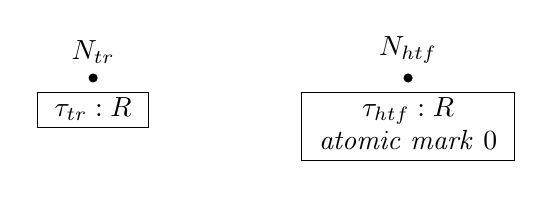
\begin{tikzpicture}[yscale=-1,
place/.style={circle,draw=black, fill=black, inner sep=0pt, 
              minimum size=1mm}]

 \node[place] (1st) at (1, 0) [label=above: $N_{tr}$,
                               label=below: 
            \begin{tabular}{|l|}
             \hline
             $\tau_{tr} : R$\\
             \hline
            \end{tabular}
] {};
	

\begin{scope}[xshift=4cm]
  \node[place] (1st) at (1, 0) [label=above: $N_{htf}$,
                               label=below: 
            \begin{tabular}{|c|}
              \hline
              $\tau_{htf} : R$\\
              \textit{atomic mark} 0\\
              \hline
            \end{tabular}] {};
\end{scope}


\end{tikzpicture}
\end{center}
\caption{Similarity between tr and htf}
\label{fig:SimTrHtf}
\end{figure}
For this pair of predicates, their \textit{types} are the same, that is, $\tau_{tr}=\tau_{htf}=R$. And, the similarity value between them is not directly defined in program. Then, two steps are taken afterwards,
\begin{enumerate}
 \item Return a middle result $Sim_{m}(tr,htf)=(0,u)$.
 \item Expand $tr$ and $htf$.     
 	\begin{figure}[h!]
\begin{center}
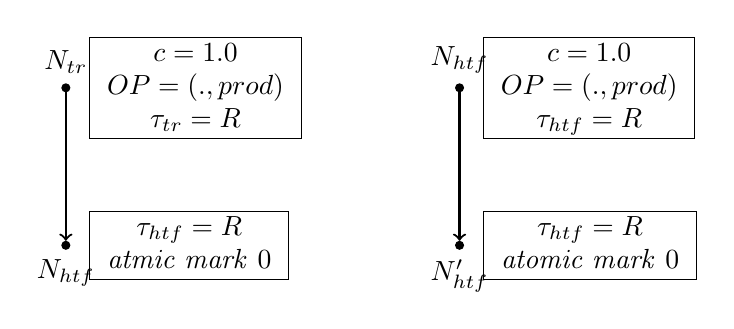
\begin{tikzpicture}[yscale=-1,
place/.style={circle,draw=black, fill=black, inner sep=0pt, 
              minimum size=1mm}]

\node[place] (1st) at (0, 0) [label=above: $N_{tr}$,
                              label=right: {
             \begin{tabular}{|c|}
               \hline
               $c=1.0$ \\
               $OP=(.,prod)$ \\
               $\tau_{tr}=R$ \\
               \hline
             \end{tabular} }] {};

\node[place] (2nd) at (0, 2) [label=below:  $N_{htf}$,
                                label=right: {
             \begin{tabular}{|c|}
               \hline
               $\tau_{htf}=R$\\
               \textit{atmic mark} $0$ \\
               \hline
             \end{tabular} }
] {};
        
	\draw[->, thick] (1st) -- (2nd);

\begin{scope}[xshift=5cm]
 \node[place] (1st) at (0, 0) [label=above: $N_{htf}$,
                              label=right: {
             \begin{tabular}{|c|}
               \hline
               $c=1.0$ \\
               $OP=(.,prod)$ \\
               $\tau_{htf}=R$ \\
               \hline
             \end{tabular} }] {};

\node[place] (2nd) at (0, 2) [label=below:  $N'_{htf}$,
                                label=right: {
             \begin{tabular}{|c|}
               \hline
               $\tau_{htf}=R$\\
               \textit{atomic mark} $0$\\
               \hline
             \end{tabular} }
] {};
        
	\draw[->, thick] (1st) -- (2nd);
\end{scope}

\end{tikzpicture}
\end{center}
\caption{Expansion of tr and htf}
\label{fig:ExpansionTrHtf}   
\end{figure} 
       According to the rule in program, which is 
       \begin{center}
         $tasty\_restaurant(X) \stackrel{1.0,.}{\longleftarrow} prod$ $has\_tasty\_food(X)$
       \end{center}
       $tr$ is expanded on the left of the figure \ref{fig:ExpansionTrHtf}, and according to $OP=(.,prod)$ from $tr$'s rule, $htf$ is expanded on the right side. As seen in the graph, only one combination of predicates in level $-1$ can be achieved, which is $(htf, htf)$. The similarity value of them is $(-1,1)$, since they are the same predicate, the similarity between them is $1$.  
\end{enumerate}
Thus, the similarity value is $1$ between $has\_tasty\_food$ and $tasty\_restaurant$ achieved in the level $-1$.

 \item $Sim(tasty\_restaurant,good\_restaurant)$
 
Since $tasty\_restaurant \in CP$, and so is $good\_restaurant$, the procedure of obtaining similarity follows the case ``complex predicate VS complex predicate''.
In an abbreviation, $tr$ is represented as $tasty\_restaurant$, $gr$ is for $good\_restaurant$, $R$ means `Restaurant'.
\begin{figure}[h!]
\begin{center}
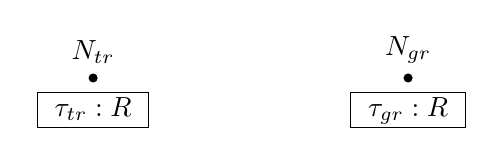
\begin{tikzpicture}[yscale=-1,
place/.style={circle,draw=black, fill=black, inner sep=0pt, 
              minimum size=1mm}]

 \node[place] (1st) at (1, 0) [label=above: $N_{tr}$,
                               label=below: 
            \begin{tabular}{|l|}
             \hline
             $\tau_{tr} : R$\\
             \hline
            \end{tabular}
] {};
	

\begin{scope}[xshift=4cm]
  \node[place] (1st) at (1, 0) [label=above: $N_{gr}$,
                               label=below: 
            \begin{tabular}{|c|}
              \hline
              $\tau_{gr} : R$\\
              \hline
            \end{tabular}] {};
\end{scope}


\end{tikzpicture}
\end{center}
\caption{Similarity between tr and gr} 
\label{fig:SimTrGr}  
\end{figure}
For this pair of predicates, their \textit{types} are the same, that is, $\tau_{tr}=\tau_{gr}=R$. And, the similarity value between them is not directly defined in RFuzzy program. Then, two steps are taken afterwards,
\begin{enumerate}
 \item Return a middle result $Sim_{m}(tr,gr)=(0,u)$.
 \item Expand $tr$ and $gr$. 
      \begin{figure}[h!]
\begin{center}
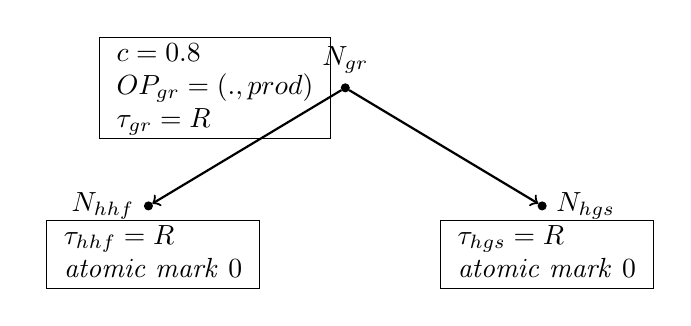
\begin{tikzpicture}[yscale=-1,
place/.style={circle,draw=black, fill=black, inner sep=0pt, 
              minimum size=1mm}]

  \node[place] (1st) at (2.5, 0) [label=above: $N_{gr}$,
                                  label=left: { 
             \begin{tabular}{|l|}
               \hline
               $c=0.8$\\
               $OP_{gr}=(.,prod)$\\
               $\tau_{gr}=R$\\
               \hline
             \end{tabular} }
] {};
	\node[place] (2nd) at (0, 1.5) [label=left: $N_{hhf}$,
                                        label=below: {
              \begin{tabular}{|l|}
                \hline
                 $\tau_{hhf}=R$ \\
                 \textit{atomic mark} $0$ \\
                \hline
              \end{tabular} }
             ] {};

        \node[place] (3rd) at (5, 1.5) [label=right: $N_{hgs}$, 
                                        label=below: {
              \begin{tabular}{|l|}
               \hline
               $\tau_{hgs}=R$ \\
               \textit{atomic mark} $0$ \\
               \hline
              \end{tabular} }
] {}; 

	\draw[->, thick] (1st) -- (2nd);
        \draw[->, thick] (1st) -- (3rd);
\end{tikzpicture}
\end{center}
\caption{Expansion of gr}
\label{fig:ExpansionGr}   
\end{figure}
       $gr$ is expanded acccording to the rule in program, which is 
      \begin{center}
       $good\_restaurant(X) \stackrel{0.8,.}{\longleftarrow} prod$ $has\_healthy\_food(X), has\_good\_service(X)$ 
      \end{center}
      According to the rule
      \begin{center}
         $tasty\_restaurant(X) \stackrel{1.0,.}{\longleftarrow} prod$ $has\_tasty\_food(X)$
      \end{center}
      and equivalence extension associated with $OP_{gr}$, the $tr$ is expanded into,
      \begin{figure}[h!]
\begin{center}
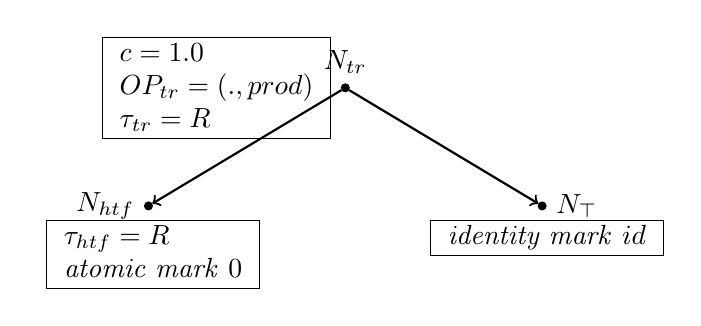
\begin{tikzpicture}[yscale=-1,
place/.style={circle,draw=black, fill=black, inner sep=0pt, 
              minimum size=1mm}]

  \node[place] (1st) at (2.5, 0) [label=above: $N_{tr}$,
                                  label=left: { 
             \begin{tabular}{|l|}
               \hline
               $c=1.0$\\
               $OP_{tr}=(.,prod)$\\
               $\tau_{tr}=R$\\
               \hline
             \end{tabular} }
] {};
	\node[place] (2nd) at (0, 1.5) [label=left: $N_{htf}$,
                                        label=below: {
              \begin{tabular}{|l|}
                \hline
                 $\tau_{htf}=R$ \\
                 \textit{atomic mark} $0$ \\
                \hline
              \end{tabular} }
             ] {};

        \node[place] (3rd) at (5, 1.5) [label=right: $N_{\top}$, 
                                        label=below: {
              \begin{tabular}{|l|}
               \hline
               \textit{identity mark} $id$ \\
               \hline
              \end{tabular} }
] {}; 

	\draw[->, thick] (1st) -- (2nd);
        \draw[->, thick] (1st) -- (3rd);
\end{tikzpicture}
\end{center}
\caption{Expansion of tr}
\label{fig:ExpansionTr}   
\end{figure}
       Two combinations of predicates in level $-1$ can be achieved, which are $M_{s_1}=\{(hhf,htf),(hgs,\top)\}$ and $M_{s_2}=\{(hgs,htf),(hhf,\top)\}$. In our program, only similarity between $has\_tasty\_food$ and $has\_healthy\_food$ is defined as \[Sim(has\_healthy\_food, has\_tasty\_food) = 0.6\]
       Suppose that for any predicate $p$, $Sim(\top,p)=0.5$, then the similarity achieved from $M_{s_1}$ is $M_{r_1}=(-1,0.6\dot{3})$ and from $M_{s_1}$ is $M_{r_2}=(-1,0.4\dot{3})$. The former combination $M_{s_1}$ will be chosen. In $M_{s_1}$, there is no $(l,u)$, which means no undefined similarity in this level $l$. Thus the comparing trees are \textit{completely built}, the algorithm terminates, and the similarity value is $0.63$ between $good\_restaurant$ and $tasty\_restaurant$ achieved in the level $-1$.       .  
\end{enumerate}

\end{itemize}



\subsection{Complexity of algorithm}
\label{sec:Complexity}
The similarity algorithm is a procedure of comparison and extension alternatively until the predicates are not necessary to or can not be expanded. For each pair of predicates $(p_i,p_j)$, it could be expanded $n_i \times n_j$ different comparing trees, where $n_i$ is the number of the rules with $p_i$ as head, and $n_j$ is the number of the rules with $p_j$ as head. The complexity of calculating the middle result for each level is
constant, since the number of children from $p_i$ or $p_j$ is constant.
The maximum number of comparison and extension is the level of the comparing trees which are \textit{completely built}, which is less than the number of rules, since one rule associates one expansion, and there are some different rules for one predicate. Suppose that the number of rules in the RFuzzy Program is $n$, then the complexity of similarity algorithm is approximatively $n_i \cdot n_j \cdot c_1 \cdot c_2 \cdot n$, where the $n_i
\cdot n_j$ is the number of possible expansion of comparing $p_i$ and $p_j$, $c_1$ is the number of nodes on one level, which is a constant, and $c_2$ is the number of comparing times for one level to achieve the middle result, and is also a constant. $n$ is represented as the number of levels. The complexity of algorithm is less than $\mathcal{O}(n^3)$.
